% A lozenge tiling of the hexagon with sides 4, 5, 3 (a plane partition in a 4x5x3 box).
% The lozenges with vertical edges form 3 chains from the left vertical side to the right one.
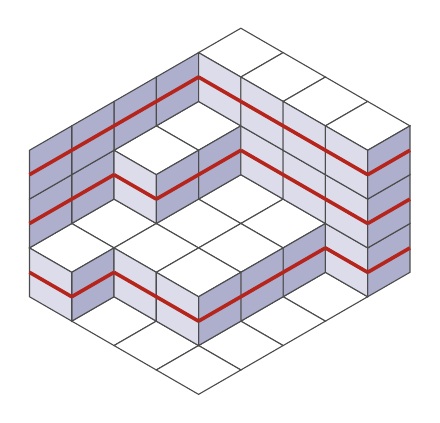
\begin{tikzpicture}[scale=0.62]
\filldraw[fill=white,draw=black!70,line width=0.4pt] (0.000,3.000)--(0.866,2.500)--(0.000,2.000)--(-0.866,2.500)--cycle;
\filldraw[fill=white,draw=black!70,line width=0.4pt] (-0.866,1.500)--(0.000,1.000)--(-0.866,0.500)--(-1.732,1.000)--cycle;
\filldraw[fill=white,draw=black!70,line width=0.4pt] (-1.732,1.000)--(-0.866,0.500)--(-1.732,0.000)--(-2.598,0.500)--cycle;
\filldraw[fill=white,draw=black!70,line width=0.4pt] (-2.598,-0.500)--(-1.732,-1.000)--(-2.598,-1.500)--(-3.464,-1.000)--cycle;
\filldraw[fill=white,draw=black!70,line width=0.4pt] (-3.464,-1.000)--(-2.598,-1.500)--(-3.464,-2.000)--(-4.330,-1.500)--cycle;
\filldraw[fill=white,draw=black!70,line width=0.4pt] (0.866,2.500)--(1.732,2.000)--(0.866,1.500)--(0.000,2.000)--cycle;
\filldraw[fill=white,draw=black!70,line width=0.4pt] (0.000,0.000)--(0.866,-0.500)--(0.000,-1.000)--(-0.866,-0.500)--cycle;
\filldraw[fill=white,draw=black!70,line width=0.4pt] (-0.866,-0.500)--(0.000,-1.000)--(-0.866,-1.500)--(-1.732,-1.000)--cycle;
\filldraw[fill=white,draw=black!70,line width=0.4pt] (-1.732,-1.000)--(-0.866,-1.500)--(-1.732,-2.000)--(-2.598,-1.500)--cycle;
\filldraw[fill=white,draw=black!70,line width=0.4pt] (-2.598,-2.500)--(-1.732,-3.000)--(-2.598,-3.500)--(-3.464,-3.000)--cycle;
\filldraw[fill=white,draw=black!70,line width=0.4pt] (1.732,2.000)--(2.598,1.500)--(1.732,1.000)--(0.866,1.500)--cycle;
\filldraw[fill=white,draw=black!70,line width=0.4pt] (0.866,-0.500)--(1.732,-1.000)--(0.866,-1.500)--(0.000,-1.000)--cycle;
\filldraw[fill=white,draw=black!70,line width=0.4pt] (0.000,-1.000)--(0.866,-1.500)--(0.000,-2.000)--(-0.866,-1.500)--cycle;
\filldraw[fill=white,draw=black!70,line width=0.4pt] (-0.866,-1.500)--(0.000,-2.000)--(-0.866,-2.500)--(-1.732,-2.000)--cycle;
\filldraw[fill=white,draw=black!70,line width=0.4pt] (-1.732,-3.000)--(-0.866,-3.500)--(-1.732,-4.000)--(-2.598,-3.500)--cycle;
\filldraw[fill=white,draw=black!70,line width=0.4pt] (2.598,1.500)--(3.464,1.000)--(2.598,0.500)--(1.732,1.000)--cycle;
\filldraw[fill=white,draw=black!70,line width=0.4pt] (1.732,-2.000)--(2.598,-2.500)--(1.732,-3.000)--(0.866,-2.500)--cycle;
\filldraw[fill=white,draw=black!70,line width=0.4pt] (0.866,-2.500)--(1.732,-3.000)--(0.866,-3.500)--(0.000,-3.000)--cycle;
\filldraw[fill=white,draw=black!70,line width=0.4pt] (0.000,-3.000)--(0.866,-3.500)--(0.000,-4.000)--(-0.866,-3.500)--cycle;
\filldraw[fill=white,draw=black!70,line width=0.4pt] (-0.866,-3.500)--(0.000,-4.000)--(-0.866,-4.500)--(-1.732,-4.000)--cycle;
\filldraw[fill=MidnightBlue!35,draw=black!70,line width=0.4pt] (-0.866,1.500)--(-1.732,1.000)--(-1.732,2.000)--(-0.866,2.500)--cycle;
\filldraw[fill=MidnightBlue!35,draw=black!70,line width=0.4pt] (-1.732,1.000)--(-2.598,0.500)--(-2.598,1.500)--(-1.732,2.000)--cycle;
\filldraw[fill=MidnightBlue!35,draw=black!70,line width=0.4pt] (-2.598,-0.500)--(-3.464,-1.000)--(-3.464,0.000)--(-2.598,0.500)--cycle;
\filldraw[fill=MidnightBlue!35,draw=black!70,line width=0.4pt] (-2.598,0.500)--(-3.464,0.000)--(-3.464,1.000)--(-2.598,1.500)--cycle;
\filldraw[fill=MidnightBlue!35,draw=black!70,line width=0.4pt] (-3.464,-1.000)--(-4.330,-1.500)--(-4.330,-0.500)--(-3.464,0.000)--cycle;
\filldraw[fill=MidnightBlue!35,draw=black!70,line width=0.4pt] (-3.464,0.000)--(-4.330,-0.500)--(-4.330,0.500)--(-3.464,1.000)--cycle;
\filldraw[fill=MidnightBlue!35,draw=black!70,line width=0.4pt] (0.000,0.000)--(-0.866,-0.500)--(-0.866,0.500)--(0.000,1.000)--cycle;
\filldraw[fill=MidnightBlue!35,draw=black!70,line width=0.4pt] (-0.866,-0.500)--(-1.732,-1.000)--(-1.732,0.000)--(-0.866,0.500)--cycle;
\filldraw[fill=MidnightBlue!35,draw=black!70,line width=0.4pt] (-2.598,-2.500)--(-3.464,-3.000)--(-3.464,-2.000)--(-2.598,-1.500)--cycle;
\filldraw[fill=MidnightBlue!35,draw=black!70,line width=0.4pt] (1.732,-2.000)--(0.866,-2.500)--(0.866,-1.500)--(1.732,-1.000)--cycle;
\filldraw[fill=MidnightBlue!35,draw=black!70,line width=0.4pt] (0.866,-2.500)--(0.000,-3.000)--(0.000,-2.000)--(0.866,-1.500)--cycle;
\filldraw[fill=MidnightBlue!35,draw=black!70,line width=0.4pt] (0.000,-3.000)--(-0.866,-3.500)--(-0.866,-2.500)--(0.000,-2.000)--cycle;
\filldraw[fill=MidnightBlue!35,draw=black!70,line width=0.4pt] (3.464,-2.000)--(2.598,-2.500)--(2.598,-1.500)--(3.464,-1.000)--cycle;
\filldraw[fill=MidnightBlue!35,draw=black!70,line width=0.4pt] (3.464,-1.000)--(2.598,-1.500)--(2.598,-0.500)--(3.464,0.000)--cycle;
\filldraw[fill=MidnightBlue!35,draw=black!70,line width=0.4pt] (3.464,0.000)--(2.598,-0.500)--(2.598,0.500)--(3.464,1.000)--cycle;
\filldraw[fill=MidnightBlue!15,draw=black!70,line width=0.4pt] (-0.866,1.500)--(0.000,1.000)--(0.000,2.000)--(-0.866,2.500)--cycle;
\filldraw[fill=MidnightBlue!15,draw=black!70,line width=0.4pt] (0.000,0.000)--(0.866,-0.500)--(0.866,0.500)--(0.000,1.000)--cycle;
\filldraw[fill=MidnightBlue!15,draw=black!70,line width=0.4pt] (0.000,1.000)--(0.866,0.500)--(0.866,1.500)--(0.000,2.000)--cycle;
\filldraw[fill=MidnightBlue!15,draw=black!70,line width=0.4pt] (0.866,-0.500)--(1.732,-1.000)--(1.732,0.000)--(0.866,0.500)--cycle;
\filldraw[fill=MidnightBlue!15,draw=black!70,line width=0.4pt] (0.866,0.500)--(1.732,0.000)--(1.732,1.000)--(0.866,1.500)--cycle;
\filldraw[fill=MidnightBlue!15,draw=black!70,line width=0.4pt] (1.732,-2.000)--(2.598,-2.500)--(2.598,-1.500)--(1.732,-1.000)--cycle;
\filldraw[fill=MidnightBlue!15,draw=black!70,line width=0.4pt] (1.732,-1.000)--(2.598,-1.500)--(2.598,-0.500)--(1.732,0.000)--cycle;
\filldraw[fill=MidnightBlue!15,draw=black!70,line width=0.4pt] (1.732,0.000)--(2.598,-0.500)--(2.598,0.500)--(1.732,1.000)--cycle;
\filldraw[fill=MidnightBlue!15,draw=black!70,line width=0.4pt] (-2.598,-0.500)--(-1.732,-1.000)--(-1.732,0.000)--(-2.598,0.500)--cycle;
\filldraw[fill=MidnightBlue!15,draw=black!70,line width=0.4pt] (-2.598,-2.500)--(-1.732,-3.000)--(-1.732,-2.000)--(-2.598,-1.500)--cycle;
\filldraw[fill=MidnightBlue!15,draw=black!70,line width=0.4pt] (-1.732,-3.000)--(-0.866,-3.500)--(-0.866,-2.500)--(-1.732,-2.000)--cycle;
\filldraw[fill=MidnightBlue!15,draw=black!70,line width=0.4pt] (-4.330,-2.500)--(-3.464,-3.000)--(-3.464,-2.000)--(-4.330,-1.500)--cycle;
\draw[BrickRed,line width=1.3pt] (-0.866,2.000)--(-1.732,1.500);
\draw[BrickRed,line width=1.3pt] (-1.732,1.500)--(-2.598,1.000);
\draw[BrickRed,line width=1.3pt] (-2.598,0.000)--(-3.464,-0.500);
\draw[BrickRed,line width=1.3pt] (-2.598,1.000)--(-3.464,0.500);
\draw[BrickRed,line width=1.3pt] (-3.464,-0.500)--(-4.330,-1.000);
\draw[BrickRed,line width=1.3pt] (-3.464,0.500)--(-4.330,0.000);
\draw[BrickRed,line width=1.3pt] (0.000,0.500)--(-0.866,0.000);
\draw[BrickRed,line width=1.3pt] (-0.866,0.000)--(-1.732,-0.500);
\draw[BrickRed,line width=1.3pt] (-2.598,-2.000)--(-3.464,-2.500);
\draw[BrickRed,line width=1.3pt] (1.732,-1.500)--(0.866,-2.000);
\draw[BrickRed,line width=1.3pt] (0.866,-2.000)--(0.000,-2.500);
\draw[BrickRed,line width=1.3pt] (0.000,-2.500)--(-0.866,-3.000);
\draw[BrickRed,line width=1.3pt] (3.464,-1.500)--(2.598,-2.000);
\draw[BrickRed,line width=1.3pt] (3.464,-0.500)--(2.598,-1.000);
\draw[BrickRed,line width=1.3pt] (3.464,0.500)--(2.598,0.000);
\draw[BrickRed,line width=1.3pt] (-0.866,2.000)--(0.000,1.500);
\draw[BrickRed,line width=1.3pt] (0.000,0.500)--(0.866,0.000);
\draw[BrickRed,line width=1.3pt] (0.000,1.500)--(0.866,1.000);
\draw[BrickRed,line width=1.3pt] (0.866,0.000)--(1.732,-0.500);
\draw[BrickRed,line width=1.3pt] (0.866,1.000)--(1.732,0.500);
\draw[BrickRed,line width=1.3pt] (1.732,-1.500)--(2.598,-2.000);
\draw[BrickRed,line width=1.3pt] (1.732,-0.500)--(2.598,-1.000);
\draw[BrickRed,line width=1.3pt] (1.732,0.500)--(2.598,0.000);
\draw[BrickRed,line width=1.3pt] (-2.598,0.000)--(-1.732,-0.500);
\draw[BrickRed,line width=1.3pt] (-2.598,-2.000)--(-1.732,-2.500);
\draw[BrickRed,line width=1.3pt] (-1.732,-2.500)--(-0.866,-3.000);
\draw[BrickRed,line width=1.3pt] (-4.330,-2.000)--(-3.464,-2.500);
\end{tikzpicture}
